% !Mode:: "TeX:UTF-8"
\thispagestyle{empty}
\chapter{Tightly Coupled LIO System}
\label{cpt:tightly-lio}
\thispagestyle{empty}

From this chapter through the next three chapters, we will introduce readers to some practical autonomous driving localization and mapping technologies. This chapter focuses on the tightly coupled Lidar-IMU-Odometry system, known as the tightly coupled LIO system (sometimes referred to as Lins\cite{Qin2020} in literature, meaning a system combining LiDAR and inertial navigation). Chapters~\ref{cpt:mapping} and~\ref{cpt:localization} will cover offline mapping systems and real-time fusion localization techniques respectively. Overall, autonomous driving applications of SLAM primarily concentrate on two major modules: mapping and localization. Within the localization module, DR or LIO is often used for local position estimation. The tightly coupled LIO system is more complex than the loosely coupled LIO system introduced in the previous chapter. This chapter will first explain its principles before proceeding with implementation.

\includepdf[width=\textwidth]{art/ch8.pdf}

\section{Principles and Advantages of Tight Coupling}
First, let's address a fundamental question: What is tight coupling, and why do we need a tightly coupled LIO system? The loosely coupled LIO introduced in the previous chapter already demonstrates good performance - what additional benefits can tight coupling provide? In fact, the term ``\textbf{tightly coupled}'' isn't unique to LIO systems; similar concepts exist in traditional integrated navigation and VIO fields\cite{yang2019tightly,liu2018implementation,kong2015tightly}. Broadly speaking, any state estimation system that considers the intrinsic properties of sensors rather than \textbf{modularly} fusing their outputs can be called a tightly coupled system\cite{Soloviev2008}. For example, systems considering IMU observation noise and biases can be called tightly coupled IMU (or INS) systems; those accounting for LiDAR registration residuals are tightly coupled LiDAR systems; while systems incorporating visual feature reprojection errors or RTK sub-states and satellite counts qualify as tightly coupled visual or RTK systems\cite{Shi2012,Schleicher2009}. In loosely coupled systems, we can treat each sensor or algorithm module as a black box, considering only their outputs. The previous chapter demonstrated this approach, which readers should now understand.

So what specific advantages does tight coupling offer? Based on the author's experience, when all algorithm modules function normally, there may be no significant difference between tightly and loosely coupled systems. For instance, when fusing GINS systems with LiDAR odometry, if RTK signals remain valid, the coupling approach shouldn't produce noticeable differences. However, in real-world systems, individual algorithm modules often can't maintain continuous normal operation. Standalone IMU systems quickly diverge without velocity and position observations; independent LiDAR and visual odometry may fail or degrade in structurally poor environments. In loosely coupled systems, when a module fails, we must logically identify the failure and attempt recovery. Tightly coupled systems allow one module's operational status to directly influence others, helping better constrain their working dimensions. Taking loosely coupled LIO as an example: when a vehicle traverses degenerate areas, LiDAR odometry relying solely on point cloud matching may fail, producing erroneous pose estimates with extra degrees of freedom that could mislead the entire system after fusion. In tightly coupled LIO systems, states remain constrained by other sensors, keeping these degrees of freedom within fixed bounds to maintain system validity. While this explanation may seem abstract, this chapter will use practical cases to help readers better understand these concepts.

\section{LIO System Based on IEKF}  
\subsection{State Variables and Motion Equations of IEKF}  

In a tightly-coupled LIO system, the IMU and LiDAR point cloud registration share the same state model, motion equations, and observation equations. Thus, the most straightforward fusion method is to incorporate both into the EKF model, where the IMU provides constraints during motion and the LiDAR point cloud provides constraints for the observation equation. However, whether using ICP or NDT, LiDAR point cloud registration often requires multiple nearest-neighbor iterations to converge to the correct solution—a point readers should have grasped from the earlier chapters on ICP and NDT. Therefore, we must also adapt the traditional EKF filter into its iterative version: the Iterated Extended Kalman Filter (IEKF). The theory of IEKF is slightly more complex than EKF, but fortunately, we have already derived the error-state Kalman filter in Chapter~\ref{cpt:ins}. This section will focus on the iteration process and the integration of LiDAR residuals.  

First, let us revisit the ESKF theory introduced earlier. For convenience, we denote its high-dimensional state variables uniformly as $\mathbf{x}$, defined in a high-dimensional manifold space $\mathcal{M}$:  
\begin{equation}\label{eq:def-of-state-variable}  
	\mathbf{x} = [\mathbf{p}, \mathbf{v}, \mathbf{R}, \mathbf{b}_g, \mathbf{b}_a, \mathbf{g}]^\top \in \mathcal{M}.  
\end{equation}  

We know that its error state can be defined in the usual vector space, i.e., the tangent space of $\mathcal{M}$ near the operating point: $\delta \mathbf{x} \in \mathbb{R}^{18}$. When IMU data arrives, the filter propagates the state variables based on the IMU readings and the current state. The motion process consists of two parts:  

1. \textbf{State Propagation Using IMU Readings}: Given the IMU readings $\tilde{\boldsymbol{\omega}}, \tilde{\mathbf{a}}$ between time $t$ and $t+\Delta t$, the discrete-time propagation can be written as:  
\begin{subequations}\label{key}  
	\begin{align}  
		\mathbf{p}(t+\Delta t) &= \mathbf{p}(t) + \mathbf{v} \Delta t + \frac{1}{2}   
		\left(\mathbf{R}(\tilde{\mathbf{a}}-\mathbf{b}_a) \right) \Delta t^2 + \frac{1}{2} \mathbf{g} \Delta t^2, \\  
		\mathbf{v}(t+\Delta t) &= \mathbf{v}(t) + \mathbf{R} (\tilde{\mathbf{a}} - \mathbf{b}_a) \Delta t + \mathbf{g} \Delta t, \\  
		\mathbf{R}(t+\Delta t) &= \mathbf{R}(t) \mathrm{Exp} \left( (\tilde{\boldsymbol{\omega}}-\mathbf{b}_g)   
		\Delta t \right), \\  
		\mathbf{b}_g(t+\Delta t) &= \mathbf{b}_g(t), \\  
		\mathbf{b}_a(t+\Delta t) &= \mathbf{b}_a(t), \\  
		\mathbf{g}(t+\Delta t) &= \mathbf{g}(t) .  
	\end{align}  
\end{subequations}  

2. \textbf{Observation Process}: While the nominal state is updated according to the above equations, the mean of the error state remains zero, and only its covariance needs to be updated:  
\begin{equation}\label{key}  
	\mathbf{P}_{\text{pred}} = \mathbf{F} \mathbf{P} \mathbf{F}^\top + \mathbf{Q},  
\end{equation}  
where $\mathbf{Q}$ is the noise matrix, $\mathbf{P}$ is the state covariance from the previous time step, and the $\mathbf{F}$ matrix is derived from the linear form of error kinematics:  
\begin{equation}  
	\mathbf{F} = \begin{bmatrix}  
		\mathbf{I} & \mathbf{I} \Delta t & \mathbf{0} & \mathbf{0} & \mathbf{0} & \mathbf{0} \\  
		\mathbf{0} & \mathbf{I} & - \mathbf{R}(\tilde{\mathbf{a}} - \mathbf{b}_a)^\wedge \Delta t & \mathbf{0} & -\mathbf{R} \Delta t & \mathbf{I} \Delta t \\  
		\mathbf{0} & \mathbf{0} & \mathrm{Exp}\left( -(\tilde{\boldsymbol{\omega}} - \mathbf{b}_g) \Delta t \right)   
		& -\mathbf{I} \Delta t & \mathbf{0} &\mathbf{0} \\  
		\mathbf{0} & \mathbf{0} & \mathbf{0} & \mathbf{I} & \mathbf{0} & \mathbf{0} \\  
		\mathbf{0} & \mathbf{0} & \mathbf{0} & \mathbf{0} & \mathbf{I} & \mathbf{0} \\  
		\mathbf{0} & \mathbf{0} & \mathbf{0} & \mathbf{0} & \mathbf{0} & \mathbf{I}  
	\end{bmatrix}.  
\end{equation}  

These details were introduced earlier (see Equation~\eqref{eq:eskf-F}). For the reader's convenience, they are restated here. Since the LiDAR frequency is typically lower than the IMU frequency, multiple IMU readings may exist between two LiDAR data points. We simply propagate the state multiple times using the above equations. For brevity, we omit subscripts and superscripts for multiple propagation steps and denote the propagated state estimate as $\mathbf{x}_{\mathrm{pred}}, \mathbf{P}_{\mathrm{pred}}$. Before applying the observation equation for correction, the estimated mean and covariance are these two quantities.

\subsection{Iterative Process in the Observation Equation}  

In a tightly-coupled system, we incorporate the ICP or NDT residuals from the LiDAR as observation equations into the EKF model. However, since both ICP and NDT require iterations to converge, we should also introduce an \textbf{iterative process} for the EKF observation step. This iterative process has the following key points:  

1. \textbf{Linearization of the Error State}: The iterative process first \textbf{linearizes} the \textbf{error state}. That is, the nominal state starts from \(\mathbf{x}_{\mathrm{pred}}\) and is continuously updated by the error state \(\delta \mathbf{x}\). Since the update \(\delta \mathbf{x}\) varies with each iteration, we denote the error state at the \(k\)-th iteration as \(\delta \mathbf{x}_k\) and its covariance as \(\mathbf{P}_k\)\footnote{Note that in Chapter 3 of this book, the subscript \(k\) was used to denote the \(k\)-th time step. Here, however, we focus on the state within a single time step and use \(k\) to represent the iteration count rather than the time step. Adding additional superscripts or subscripts for iterations would make the notation overly cumbersome.}. At \(k=0\), we initialize the process as: \(\delta \mathbf{x}_{0} = \mathbf{0}, \mathbf{P}_0 = \mathbf{P}_{\mathrm{pred}}\).  

2. \textbf{Recomputing Kalman Gain and Update}: Since the observation equation requires iteration, the Kalman gain and update process must also be recomputed at each step. Thus, quantities related to the update are also subscripted with \(k\), denoted as \(\mathbf{K}_k, \mathbf{H}_k\). Before updating, we denote the working point as \(\mathbf{x}_k\), which is essentially obtained by incrementally adding \(\delta \mathbf{x}_k\) to \(\mathbf{x}_0\). From the perspective of nominal and error states, the nominal state at the \(k\)-th iteration is \(\mathbf{x}_k\), while the error state is \(\mathbf{0}\).  

3. \textbf{Practical Tricks for \(\mathbf{P}\) Updates}: During IEKF iterations before convergence, we can consider the filter as still in progress, merely shifting the working point. Thus, \(\mathbf{P}\) does not need to be recalculated at every iteration—only the initial \(\mathbf{P}_{\mathrm{pred}}\) needs to be projected into the current tangent space. The final \(\mathbf{P}\) update is performed only after the last iteration, projecting it to the new working point.  

4. \textbf{Differences Due to Repeated Linearization}: In EKF, linearization is performed only once at \(\mathbf{x}_{\mathrm{pred}}\). In IEKF, however, the \(k\)-th linearization is computed at \(\mathbf{x}_k\). Traditional EKF describes how to update \(\mathbf{x}_{\mathrm{pred}}, \mathbf{P}_{\mathrm{pred}}\) to \(\mathbf{x}, \mathbf{P}\), whereas IEKF focuses on updating \(\mathbf{x}_{k-1}, \mathbf{P}_{k-1}\) to \(\mathbf{x}_{k}, \mathbf{P}_k\) (though, as noted earlier, \(\mathbf{P}_k\) does not need to be explicitly computed). This difference leads to significant variations in the update process between EKF and IEKF, which will be reflected in later implementations.  

5. \textbf{Dynamic Observation Model}: Like ICP and NDT, tightly-coupled LIO should update the nearest-neighbor relationships for each matched point in every iteration. This results in an IEKF observation model \textbf{with a variable number of equations}, unlike standard EKF, which has a fixed observation dimension\footnote{This is specific to LIO and does not imply that IEKF generally alters the number of observation equations.}. When the observation dimension is large, certain algebraic transformations are applied to EKF formulas to handle high-dimensional computations.  

The overall process is illustrated in Figure~\ref{fig:iekf-iters}. Starting from \(\mathbf{x}_0, \mathbf{P}_0\), we iteratively refine the observation model, compute the incremental update \(\delta \mathbf{x}\), and update \(\mathbf{x}\) and \(\mathbf{P}\) until convergence.  

\begin{figure}[!htp]  
	\centering  
	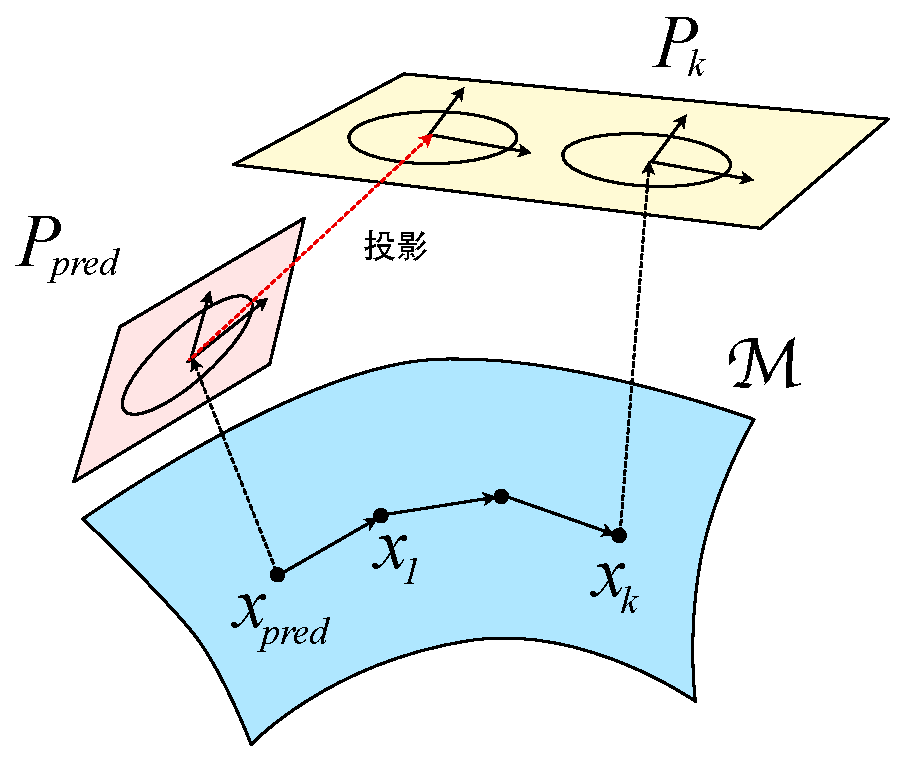
\includegraphics[width=0.5\textwidth]{resources/lio/iekf-iters.pdf}  
	\caption{Schematic diagram of the Iterated Kalman Filter}  
	\label{fig:iekf-iters}  
\end{figure}  

Next, we derive this process. Consider the \(k\)-th iteration, where the working point is \(\mathbf{x}_{k}, \mathbf{P}_{k}\), and we aim to compute the incremental update \(\delta \mathbf{x}_{k+1}\). First, we clarify the relationship between \(\mathbf{x}_{k}, \mathbf{P}_{k}\) and \(\mathbf{x}_0, \mathbf{P}_0\). While \(\mathbf{x}_{k}\) is straightforward (obtained by accumulating incremental updates), \(\mathbf{P}_{k}\) requires a tangent space projection, as discussed in Chapter~\ref{cpt:ins} and Equation~\eqref{eq:tangent-space-projection}. We denote the tangent space Jacobian at the \(k\)-th iteration as \(\mathbf{J}_k\):  
\begin{equation}\label{key}  
	\mathbf{J}_k = \mathrm{diag}(\mathbf{I}_3, \mathbf{I}_3, \mathbf{J}_{\boldsymbol{\theta}}, \mathbf{I}_3, \mathbf{I}_3, \mathbf{I}_3), \quad \mathbf{J}_{\boldsymbol{\theta}} = \mathbf{I} - \frac{1}{2} \delta \boldsymbol{\theta}_k^\wedge, \quad \delta \boldsymbol{\theta}_k = \mathrm{Log}(\mathbf{R}_0^\top \mathbf{R}_k).  
\end{equation}  

This \(\mathbf{J}_k\) describes the transformation from \(\mathbf{P}_{\mathrm{pred}}\) to \(\mathbf{P}_k\). Thus, from the perspective of \(\mathbf{x}_{k}\), the prior distribution is:  
\begin{equation}\label{key}  
	\delta \mathbf{x}_k \sim \mathcal{N}(\mathbf{0}, \mathbf{J}_k \mathbf{P}_{\mathrm{pred}} \mathbf{J}_k^\top).  
\end{equation}  

We denote \(\mathbf{P}_k = \mathbf{J}_k \mathbf{P}_{\mathrm{pred}} \mathbf{J}_k^\top\). The observation model for iterative EKF is the same as standard EKF. Referring to the EKF update formula~\eqref{eq:eskf-obs-correction}, the update process for the iterated Kalman filter is:  
\begin{subequations}\label{eq:ieskf-obs-correction}  
	\begin{align}  
		\mathbf{K}_k &= \mathbf{P}_{k} \mathbf{H}_k^\top(\mathbf{H}_k \mathbf{P}_{k}   
		\mathbf{H}_k^\top + \mathbf{V})^{-1} ,\\  
		\delta \mathbf{x}_k &= \mathbf{K}_k (\mathbf{z} - \mathbf{h}(\mathbf{x}_k)).  
	\end{align}  
\end{subequations}  

If the filter has not yet converged, \(\mathbf{P}\) is not updated—instead, \(\mathbf{J}_{k+1}\) is computed from \(\mathbf{x}_{k+1}\), and the initial distribution is projected accordingly. Upon convergence, \(\mathbf{P}_{k+1}\) is updated using the Kalman formula:  
\begin{equation}\label{eq:update-of-iekf}  
	\mathbf{P}_{k+1} = (\mathbf{I} - \mathbf{K}_k \mathbf{H}_k)\mathbf{J}_k \mathbf{P}_{\mathrm{pred}} \mathbf{J}_k^\top.  
\end{equation}  

In other words, from a covariance perspective, \textbf{only the final iteration} is considered effective. The Kalman gain \(\mathbf{K}_k\) and linearization matrix \(\mathbf{H}_k\) influence only the last update. Intermediate iterations merely adjust the starting point.  

If IEKF completes the iteration, \(\mathbf{P}_{k+1}\) should also be projected into the tangent space at the final step to maintain consistency. Overall, each IEKF iteration solves a least-squares problem with a prior:  
\begin{equation}\label{key}  
	\delta \mathbf{x}_k = \arg \min\limits_{\delta \mathbf{x}} \| \mathbf{z} - \mathbf{H}_k(\mathbf{x}_k \boxplus \delta \mathbf{x}) \|_{\mathbf{V}}^2 + \| \delta \mathbf{x}_k \|_{\mathbf{P}_k}^2.  
\end{equation}  

The first term represents the observation residual, while the second term is the prior residual projected into the tangent space. This derivation differs slightly from similar works (e.g.,~\cite{he2021kalman,Barfoot2016}) but is simpler overall. A full implementation would update \(\mathbf{P}_k\) at every iteration rather than projecting \(\mathbf{P}_{\mathrm{pred}}\), but this would complicate the notation. Alternatively, all increments and covariances could be considered at \(\mathbf{x}_0\), but this would make the mathematics even more involved.

\subsection{Efficient Handling of High-Dimensional Observations}  

In tightly-coupled systems, we directly incorporate NDT or ICP residuals into the observation equation, which significantly increases the dimensionality of the observation space. In traditional integrated navigation systems like RTK, observation equations are typically 3D or 6D. However, when point clouds are included, the observation equation can easily reach thousands or even tens of thousands of dimensions. If we compute the Kalman gain using Equation~\eqref{eq:ieskf-obs-correction}(a), we inevitably encounter the inversion of a very large matrix. Suppose the residual dimension is \( m \), then \(\mathbf{H}_k\) becomes an \( m \times 18 \) matrix, and the term \((\mathbf{H}_k \mathbf{P}_{k} \mathbf{H}_k^\top + \mathbf{V})\) in the Kalman gain requires the inversion of an \( m \times m \) matrix—an operation we must avoid.  

In Kalman filters, the \textbf{Sherman-Morrison-Woodbury (SMW) identity} \cite{Sherman1950,Barfoot2016} is a widely used algebraic transformation that proves highly useful in various Kalman filter derivations. The SMW identity has four equivalent forms, one of which is:  
\begin{equation}\label{key}  
	\mathbf{A} \mathbf{B} (\mathbf{D} + \mathbf{C} \mathbf{A} \mathbf{B})^{-1} = (\mathbf{A}^{-1} + \mathbf{B} \mathbf{D}^{-1} \mathbf{C})^{-1} \mathbf{B} \mathbf{D}^{-1},  
\end{equation}  
where \(\mathbf{A}, \mathbf{B}, \mathbf{C}, \mathbf{D}\) are matrix blocks satisfying standard matrix multiplication rules. Substituting \(\mathbf{P}_k, \mathbf{H}_k, \mathbf{V}\) into this identity yields:  
\begin{equation}\label{eq:8.11}  
	\mathbf{K}_k  = (\mathbf{P}_k^{-1} + \mathbf{H}_k^\top \mathbf{V}^{-1} \mathbf{H}_k)^{-1} \mathbf{H}_k^\top \mathbf{V}^{-1}.  
\end{equation}  

Note that the inversion inside this formula is now \( 18 \times 18 \), drastically reducing the computational burden. When dealing with high-dimensional observations, we should prefer this form for computing the Kalman gain. Moreover, comparing this with the linear increment equation in NDT (Equation~\eqref{eq:ndt-normal-equation}), we observe a striking similarity: The term \((\mathbf{H}_k^\top \mathbf{V}^{-1} \mathbf{H})^{-1}\) in the Kalman gain corresponds exactly to the coefficient matrix in the normal equation, while \(\mathbf{H}^\top \mathbf{V}^{-1}\) aligns with the residual term on the right-hand side of \eqref{eq:ndt-normal-equation}. This highlights the fundamental nature of the Kalman filter as a balance between prior information and observations.  

To further clarify the connection between NDT and the Kalman filter, let us examine their formulations. The Kalman filter's incremental update \(\delta \mathbf{x}_k\) is:  
\begin{equation}\label{eq:kalman-delta-x}  
	\delta \mathbf{x}_k = \mathbf{K}_k (\mathbf{z} - \mathbf{h}(\mathbf{x}_k)),  
\end{equation}  

whereas the least-squares increment in NDT or ICP is:  
\begin{equation}\label{eq:ndt-normal}  
	\sum_{i} (\mathbf{J}_i^\top \boldsymbol{\Sigma}_i^{-1} \mathbf{J}_i) \Delta \mathbf{x} = -\sum_{i} \mathbf{J}_i^\top \boldsymbol{\Sigma}^{-1}_i \mathbf{e}_i.  
\end{equation}  

Observant readers will notice the equivalence between these two equations. The matrix inversion in \eqref{eq:ndt-normal} matches the Kalman gain in \eqref{eq:8.11} when the prior is omitted. The key difference is that the Kalman gain is expressed in matrix form, while ICP or NDT uses summation notation. For later discussions on NDT-LIO, we derive how NDT residuals are incorporated into the Kalman gain. In the experimental section, we will follow this derivation rather than the matrix-based Kalman gain.  

Consider the NDT registration of a point cloud with \( N \) points. For the \( j \)-th point, its residual \(\mathbf{r}_j\) is computed based on the voxel it falls into in the target point cloud, with an associated information matrix \(\boldsymbol{\Sigma}^{-1}_j\) (the inverse covariance of the voxel's Gaussian distribution). The squared error \(\mathbf{e}_j\) is:  
\begin{equation}\label{key}  
	\mathbf{e}_j = \mathbf{r}_j^\top \boldsymbol{\Sigma}^{-1}_j \mathbf{r}_j.  
\end{equation}  

The Jacobian of \(\mathbf{r}_j\) with respect to rotation and translation is:  
\begin{equation}\label{key}  
	\frac{\partial \mathbf{r}_j}{\partial \mathbf{R}} = -\mathbf{R} \mathbf{q}_j^\wedge, \quad \frac{\partial \mathbf{r}_j}{\partial \mathbf{t}} = \mathbf{I}.  
\end{equation}  
Following the state variable definition in \eqref{eq:def-of-state-variable}, we expand the Jacobian to match the state dimensions:  
\begin{equation}\label{key}  
	\mathbf{J}_j = \left[\frac{\partial \mathbf{r}_j}{\partial \mathbf{t}}, \mathbf{0}_{3}, \frac{\partial \mathbf{r}_j}{\partial \mathbf{R}}, \mathbf{0}_3, \mathbf{0}_3, \mathbf{0}_3 \right].  
\end{equation}  

This Jacobian was introduced in Chapter 7, and we pad it with zero blocks to align with the state vector. In the filter, the \( j \)-th block row of \(\mathbf{H}_k\)\footnote{Strictly speaking, it should be the \( 3 \times j \)-th row since \(\mathbf{J}_j\) has 3 rows. Interpreted as a block matrix, this is correct.} is \(\mathbf{J}_j\), and the noise matrix \(\mathbf{V}\) is a block-diagonal matrix composed of \(\boldsymbol{\Sigma}^{-1}_j\):  
\begin{equation}\label{key}  
	\mathbf{H}_k = \begin{bmatrix}  
		\cdots, \\  
		\mathbf{J}_j, \\  
		\cdots  
	\end{bmatrix}, \quad \mathbf{V} = \mathrm{diag}(\cdots, \boldsymbol{\Sigma}_j, \cdots).  
\end{equation}  

Since \(\mathbf{V}\) is block-diagonal, the term \(\mathbf{H}_k^\top \mathbf{V}^{-1} \mathbf{H}_k\) in the Kalman gain can be rewritten as a summation:  
\begin{equation}\label{key}  
	\mathbf{H}_k^\top \mathbf{V}^{-1} \mathbf{H}_k = \sum\limits_{j} \mathbf{J}_j^\top \boldsymbol{\Sigma}_j^{-1} \mathbf{J}_j.  
\end{equation}  

Similarly, multiplying \(\mathbf{H}_k^\top \mathbf{V}^{-1}\) by \((\mathbf{z} - \mathbf{h}(\mathbf{x}_k))\) gives:  
\begin{align}\label{key}  
	\mathbf{H}_k^\top \mathbf{V}^{-1} (\mathbf{z} - \mathbf{h}(\mathbf{x}_k)) &= \left[\cdots, \mathbf{J}_j^\top, \cdots \right] \mathrm{diag}(\cdots, \boldsymbol{\Sigma}_j^{-1}, \cdots) \begin{bmatrix}  
		\cdots \\ \mathbf{r}_j \\ \cdots  
	\end{bmatrix}, \\  
	&= \sum\limits_{j} \mathbf{J}_j^\top \boldsymbol{\Sigma}_j^{-1} \mathbf{r}_j.  
\end{align}  

For the covariance update in \eqref{eq:update-of-iekf}, substituting \(\mathbf{K}\) into \(\mathbf{I} - \mathbf{K}_k \mathbf{H}_k\) yields:  
\begin{equation}\label{key}  
	\mathbf{P}_{k+1} = (\mathbf{I} - (\mathbf{P}_k^{-1} + \mathbf{H}_k^\top \mathbf{V}^{-1} \mathbf{H}_k)^{-1} \mathbf{H}_k^\top \mathbf{V}^{-1} \mathbf{H}_k) \mathbf{J}_k \mathbf{P}_{\mathrm{pred}} \mathbf{J}_k^\top,  
\end{equation}  
where \(\mathbf{H}_k^\top \mathbf{V}^{-1} \mathbf{H}_k\) can again be replaced with the summation form from NDT. Thus, the entire iterative Kalman filter computation is tightly linked with NDT. In this sense, the tightly-coupled system can be viewed as a high-dimensional NDT or ICP with IMU predictions, where these predictions are propagated to the next time step.
\
\section{Implementation of IEKF-based LIO}
\label{sec:iekf-lio}

Next we implement the IEKF and its corresponding LIO system. As mentioned earlier, tightly-coupled LIO can compute point cloud residuals through various methods such as point-to-line, point-to-plane, NDT, etc. This section implements an NDT-LIO based on IEKF, while readers may also refer to this book or literature \cite{Bai2022,Xu2021,xu2021fast} to implement point-to-plane ICP based LIO.

We modify the ESKF from Chapter 3 to design the IEKF interface. Since we want NDT to directly provide Jacobian and information matrices, at the IEKF implementation level, we expect NDT to compute $\mathbf{H}^\top \mathbf{V}^{-1} \mathbf{H}$ and $\mathbf{H}^\top \mathbf{V}^{-1} \mathbf{r}$ (these quantities are calculated internally by NDT), then IESKF uses its return values to iterate the entire filter:

\begin{lstlisting}[language=c++,caption=src/ch8/lio-iekf/iekf.hpp]
/**
* NDT observation function, inputs an SE3 Pose, returns terms from (8.10)
* HT V^{-1} H
* H^\top V{-1} r
* Both can be done in summation form
*/
using CustomObsFunc = std::function<void(const SE3& input_pose, Eigen::Matrix<S, 18, 18>& HT_Vinv_H,
Eigen::Matrix<S, 18, 1>& HT_Vinv_r)>;

/// Update filter using custom observation function
bool UpdateUsingCustomObserve(CustomObsFunc obs) {
	SO3 start_R = R_;
	Eigen::Matrix<S, 18, 1> HTVr;
	Eigen::Matrix<S, 18, 18> HTVH;
	Eigen::Matrix<S, 18, Eigen::Dynamic> K;
	Mat18T Pk, Qk;
	
	for (int iter = 0; iter < options_.num_iterations_; ++iter) {
		// call obs function
		obs(GetNominalSE3(), HTVH, HTVr);
		
		// project P
		Mat18T J = Mat18T::Identity();
		J.template block<3, 3>(6, 6) = Mat3T::Identity() - 0.5 * SO3::hat((R_.inverse() * start_R).log());
		Pk = J * cov_ * J.transpose();
		
		// Kalman update
		Qk = (Pk.inverse() + HTVH).inverse();  // this intermediate variable can be used in final update
		dx_ = Qk * HTVr;
		LOG(INFO) << "iter " << iter << " dx = " << dx_.transpose() << ", dxn: " << dx_.norm();
		
		// merge dx into nominal variables
		UpdateAndReset();
		
		if (dx_.norm() < options_.quit_eps_) {
			break;
		}
	}
	
	// update P
	cov_ = (Mat18T::Identity() - Qk * HTVH) * Pk;
	
	// project P
	Mat18T J = Mat18T::Identity();
	J.template block<3, 3>(6, 6) = Mat3T::Identity() - 0.5 * SO3::hat(dx_.template block<3, 1>(6, 0));
	cov_ = J * cov_ * J.inverse();
	
	dx_.setZero();
	return true;
}
\end{lstlisting}

This function provides a current estimate $\mathbf{x}_k$ for external algorithms to compute the corresponding $\mathbf{H}_k^\top \mathbf{V}^{-1} \mathbf{H}_k$ and $\mathbf{H}_k^\top \mathbf{V}^{-1} \mathbf{r}_k$, which are then substituted into the IEKF calculation formula to obtain the current time increment $\delta \mathbf{x}_k$, finally applied to the nominal state variables. Note we denote $(\mathbf{P}_k^{-1} + \mathbf{H}_k^\top \mathbf{V}^{-1} \mathbf{H})^{-1}$ as intermediate variable $\mathbf{Q}_k$ in the code. This variable allows us to more simply compute the Kalman filter error state and covariance:
\begin{align}\label{key}
	\delta \mathbf{x}_k &= \mathbf{Q}_k \mathbf{H}_k^\top \mathbf{V}^{-1} \mathbf{r}_k, \\
	\mathbf{P}_{k+1} &= (\mathbf{I} - \mathbf{Q}_k \mathbf{H}^\top_k \mathbf{V}^{-1} \mathbf{H}_k) \mathbf{P}_k.
\end{align}

Following the previous derivation, we add an interface to Chapter 7's NDT to compute the corresponding matrices and return the results. The entire computation flow is completely consistent with the previous NDT, except NDT no longer needs to compute the updates itself.

\begin{lstlisting}[language=c++,caption=src/ch7/ndt\_inc.cc]
void IncNdt3d::ComputeResidualAndJacobians(const SE3& input_pose, Mat18d& HTVH, Vec18d& HTVr) {
	assert(grids_.empty() == false);
	SE3 pose = input_pose;
	
	// Most steps same as Align(), except z, H, R are handled externally
	int num_residual_per_point = 1;
	if (options_.nearby_type_ == NearbyType::NEARBY6) {
		num_residual_per_point = 7;
	}
	
	std::vector<int> index(source_->points.size());
	for (int i = 0; i < index.size(); ++i) {
		index[i] = i;
	}
	
	int total_size = index.size() * num_residual_per_point;
	
	std::vector<bool> effect_pts(total_size, false);
	std::vector<Eigen::Matrix<double, 3, 18>> jacobians(total_size);
	std::vector<Vec3d> errors(total_size);
	std::vector<Mat3d> infos(total_size);
	
	// gauss-newton iteration
	// nearest neighbor, can be parallel
	std::for_each(std::execution::par_unseq, index.begin(), index.end(), [&](int idx) {
		auto q = ToVec3d(source_->points[idx]);
		Vec3d qs = pose * q;  // transformed q
		
		// compute voxel containing qs and its neighbors
		Vec3i key = (qs * options_.inv_voxel_size_).cast<int>();
		
		for (int i = 0; i < nearby_grids_.size(); ++i) {
			Vec3i real_key = key + nearby_grids_[i];
			auto it = grids_.find(real_key);
			int real_idx = idx * num_residual_per_point + i;
			/// need to check if Gaussian distribution has been estimated
			if (it != grids_.end() && it->second.ndt_estimated_) {
				auto& v = it->second;  // voxel
				Vec3d e = qs - v.mu_;
				
				// check chi2 th
				double res = e.transpose() * v.info_ * e;
				if (std::isnan(res) || res > options_.res_outlier_th_) {
					effect_pts[real_idx] = false;
					continue;
				}
				
				// build residual
				Eigen::Matrix<double, 3, 18> J;
				J.setZero();
				J.block<3, 3>(0, 0) = Mat3d::Identity();                   // Jacobian w.r.t. p
				J.block<3, 3>(0, 6) = -pose.so3().matrix() * SO3::hat(q);  // Jacobian w.r.t. R
				
				jacobians[real_idx] = J;
				errors[real_idx] = e;
				infos[real_idx] = v.info_;
				effect_pts[real_idx] = true;
			} else {
				effect_pts[real_idx] = false;
			}
		}
	});
	
	// accumulate Hessian and error, compute dx
	double total_res = 0;
	int effective_num = 0;
	
	HTVH.setZero();
	HTVr.setZero();
	
	std::vector<double> err;
	const double info_ratio = 0.01;  // info feedback factor per point
	
	for (int idx = 0; idx < effect_pts.size(); ++idx) {
		if (!effect_pts[idx]) {
			continue;
		}
		
		total_res += errors[idx].transpose() * infos[idx] * errors[idx];
		effective_num++;
		
		err.push_back(errors[idx].transpose() * infos[idx] * errors[idx]);
		
		HTVH += jacobians[idx].transpose() * infos[idx] * jacobians[idx] * info_ratio;
		HTVr += -jacobians[idx].transpose() * infos[idx] * errors[idx] * info_ratio;
	}
}
\end{lstlisting}

Here we compute the distributions within NDT voxels in parallel, collect the Jacobians and residuals for each point, and accumulate them into the two output matrices: $\mathbf{H}_k^\top \mathbf{V}^{-1} \mathbf{H}_k$ should be an $18 \times 18$ matrix after accumulation, while $\mathbf{H}_k \mathbf{V}^{-1} \mathbf{r}_k$ should be an $18\times 1$ vector after accumulation, which readers can verify through the code. Since NDT typically has significantly more points than the prediction equation, this may bias the estimation toward NDT. We add a scaling factor (0.01) to the information matrix $\boldsymbol{\Sigma}^{-1}$ here to make the updates more balanced. Readers may adjust this parameter.

At the LIO level, we retain the loosely-coupled framework and only need to modify the registration process to the tightly-coupled form:

\begin{lstlisting}[language=c++,caption=src/ch8/lio-iekf/lio\_iekf.cc]
// subsequent scans, update using NDT with pose
ndt_.SetSource(current_scan_filter);
ieskf_.UpdateUsingCustomObserve([this](const SE3 &input_pose, Mat18d &HTVH, Vec18d &HTVr) {
	ndt_.ComputeResidualAndJacobians(input_pose, HTVH, HTVr);
});

// if moved beyond threshold, add point cloud to map
SE3 current_pose = ieskf_.GetNominalSE3();
SE3 delta_pose = last_pose_.inverse() * current_pose;
if (delta_pose.translation().norm() > 1.0 || delta_pose.so3().log().norm() > math::deg2rad(10)) {
	// merge scan into NDT map
	CloudPtr current_scan_world(new PointCloudType);
	pcl::transformPointCloud(*current_scan_filter, *current_scan_world, current_pose.matrix());
	ndt_.AddCloud(current_scan_world);
	last_pose_ = current_pose;
}
\end{lstlisting}

Internally, IEKF provides NDT with the current state estimate, NDT computes the two matrices mentioned earlier and returns them to IEKF, which then updates its internal state estimate. This gives us the pose corresponding to the current LiDAR scan. On the other hand, if the vehicle moves more than 1 meter or rotates more than 10 degrees, we merge the current LiDAR scan data into the NDT map, preventing the vehicle from continuously spending time updating the map when stationary. We can test the tightly-coupled NDT effect through this chapter's test\_lio\_iekf program. The test program displays the current point cloud and internal state variables in the UI interface.

\begin{lstlisting}[language=sh,caption=Terminal input:]
bin/test_lio_iekf --bag_path ./dataset/sad/nclt/20120115.bag --dataset_type NCLT --config ./config/velodyne_nclt.yaml
\end{lstlisting}

\begin{figure}[!htp]
	\centering
	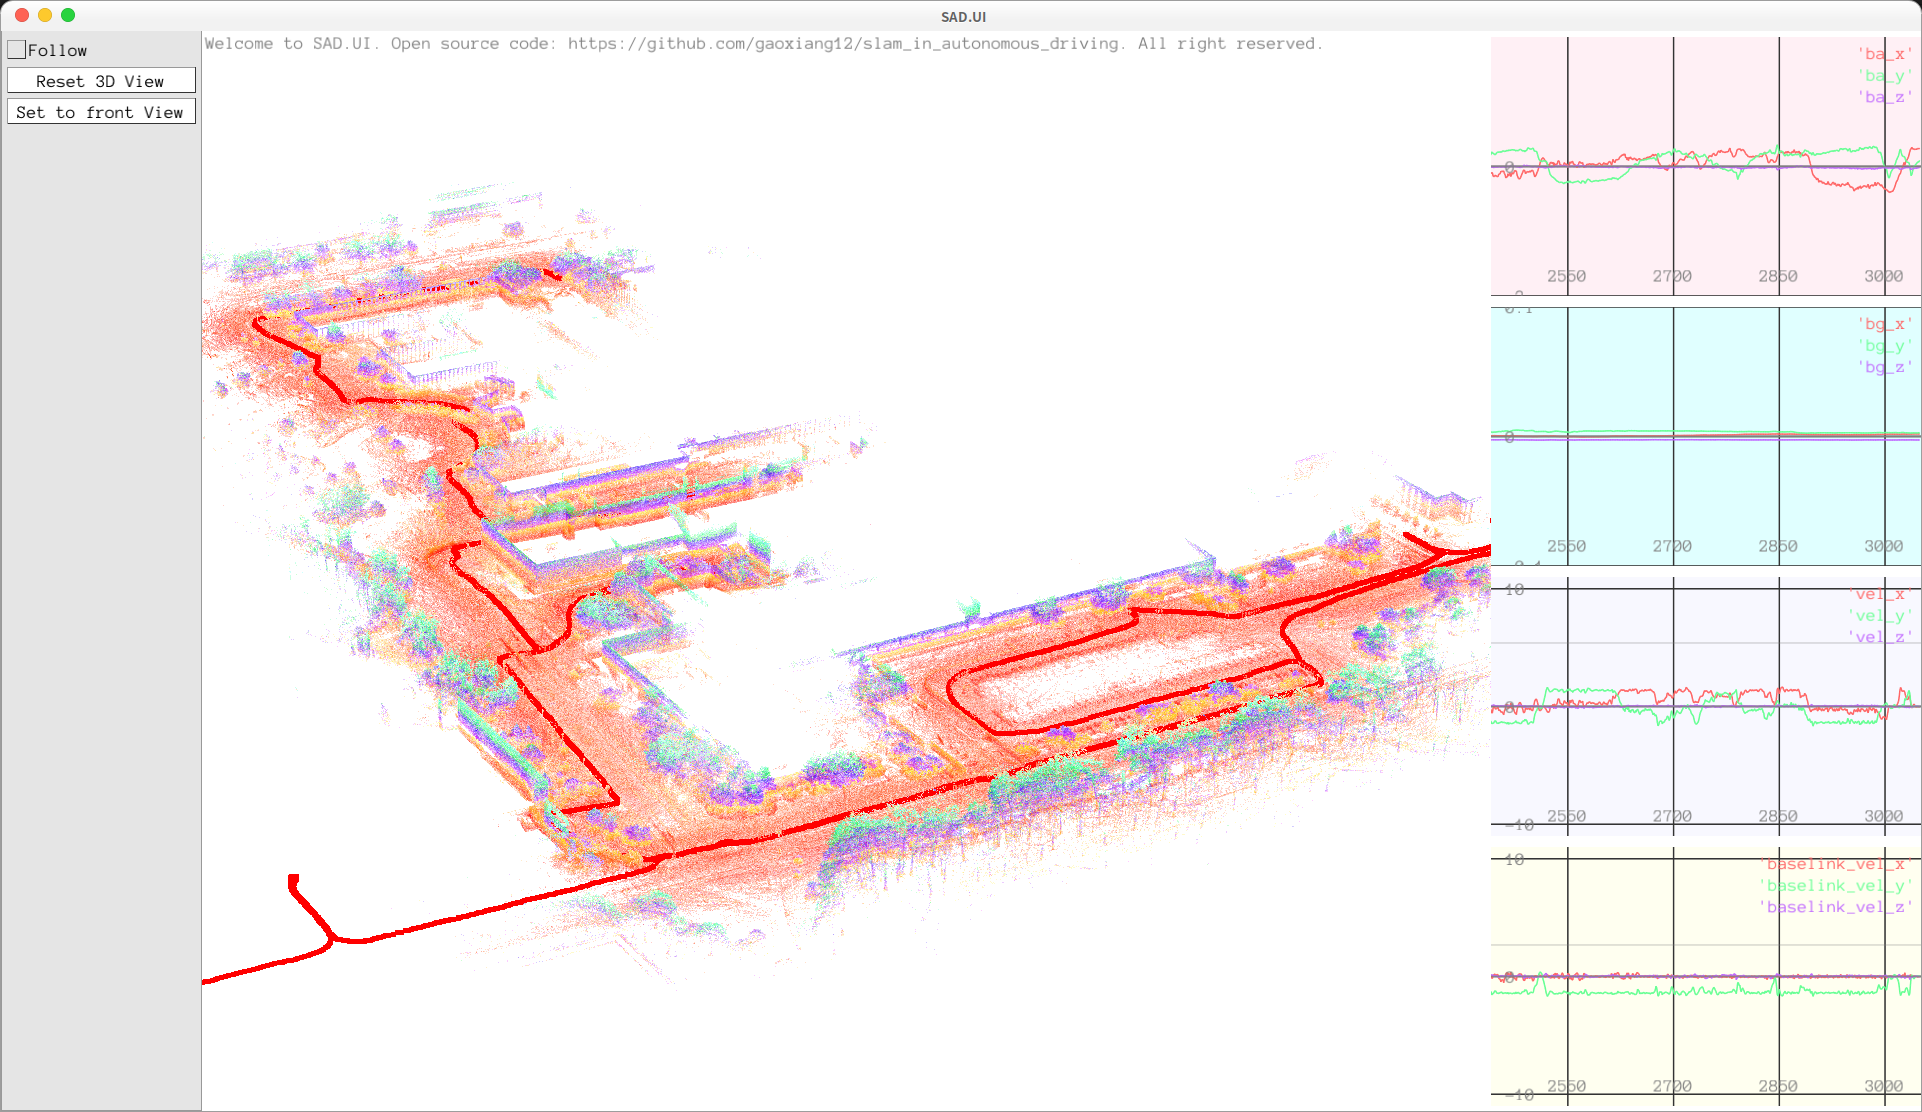
\includegraphics[width=0.8\textwidth]{resources/lio/tightly-lio.png}
	\caption{Reconstructed point cloud results from tightly-coupled LIO}
	\label{fig:tightly-lio}
\end{figure}

Readers can test this chapter's tightly-coupled LIO program on any provided dataset, with results shown in Figure~\ref{fig:tightly-lio}. Since the tightly-coupled Kalman filter iteration process is integrated with NDT, their computational efficiency is extremely high. On my machine, a single 32-beam LiDAR registration takes only 2.7 milliseconds, meaning the entire LiDAR odometry frequency can exceed 300 Hz. Traditional LiDAR odometry methods (Loam\cite{Zhang2014}, LeGo-LOAM\cite{Shan2018}, LIO-SAM\cite{Shan2020}) typically require tens or hundreds of milliseconds. The IEKF and NDT based odometry demonstrates clear advantages in computational efficiency.

\section{LIO Based on Preintegration}
\subsection{Principles of Preintegrated LIO}

Next, we introduce an LIO system based on preintegration and point cloud registration. Similar to Chapter~\ref{cpt:ins}, since we have implemented LIO using Kalman filters, we will reimplement it using preintegrated graph optimization to help readers understand their connections and differences. Like integrated navigation systems, LIO systems with LiDAR point clouds can also be implemented using preintegrated IMU factors combined with LiDAR residuals. Some modern LiDAR SLAM systems adopt this approach. Compared to filtering methods, preintegrated factors can be more conveniently integrated into existing optimization frameworks, making development and implementation easier. However, in practice, the use of preintegration is quite flexible and requires more parameter tuning than EKF systems. For example, LIO-SAM combines preintegrated factors with LiDAR odometry factors to construct the entire optimization problem \cite{Shan2020,Shan2021}. In VSLAM systems, preintegrated factors can also be combined with reprojection errors to solve Bundle Adjustment \cite{Campos2021}. Here we share some practical experience with preintegration applications:

\begin{figure}[!t]
	\centering
	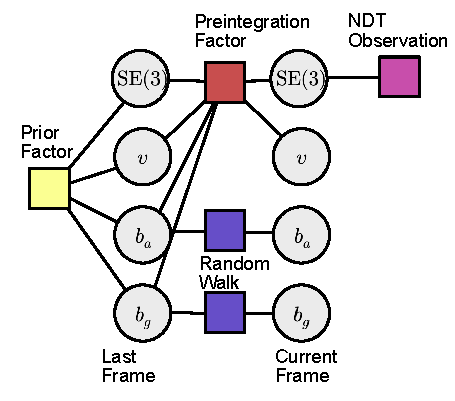
\includegraphics[width=0.4\textwidth]{resources/lio/preinteg-graph.pdf}
	\caption{Graph optimization model with preintegration}
	\label{fig:preinteg-graph}
\end{figure}

\begin{enumerate}
	\item Preintegrated factors typically connect high-dimensional states (typically 15-dimensional) between two keyframes. When converting to a graph optimization problem, we can choose to separate the vertices, e.g., having $\mathrm{SE}(3)$ as one vertex and $\mathbf{v}$ as another, with a preintegration edge connecting 8 vertices. Alternatively, we can combine the high-dimensional state into a single vertex, with preintegration edges connecting two vertices but containing many zero blocks in the Jacobian matrix. In practice, we adopt the former approach, which results in more vertex types but lower-dimensional edges.
	
	\item Since preintegrated factors involve many variables and most measurements are differences between state variables, sufficient observations and constraints on the state variables are necessary to prevent free movement in the null space. For example, the preintegrated velocity observation $\Delta \tilde{\mathbf{v}}_{ij}$ describes the difference between velocities at two keyframes. If we add a constant increment to both keyframe velocities, the velocity error remains unchanged, while adjustments to the displacement terms can keep displacement observations consistent. Therefore, in practice, we impose prior constraints on the previous keyframe and observation constraints on the subsequent keyframe to confine the optimization problem within reasonable bounds.
	
	\item The graph optimization model with preintegration is shown in Figure~\ref{fig:preinteg-graph}. When optimizing two keyframes, we add a prior factor to the previous keyframe, then include preintegration factors and bias random walk factors between the frames, and finally add NDT pose constraints to the next keyframe. After optimization, we use marginalization to compute the covariance of the next keyframe's pose, which serves as the prior factor for the next optimization round.
	
	\item This graph optimization model closely resembles the GINS system in Chapter~\ref{cpt:preinteg}. However, it's important to note that LiDAR odometry pose observations depend on prediction data, which is fundamentally different from RTK pose observations. With good RTK signals, we can assume fixed observation accuracy, ensuring convergence in both translation and rotation for filters and graph optimizers. In contrast, if LiDAR odometry uses inaccurate predicted poses, it may produce abnormal observations, causing the entire LIO to diverge. This makes debugging graph optimization-based LIO systems significantly more challenging than GINS systems.
	
	\item To reuse the code from Section~\ref{sec:iekf-lio}, we maintain the same LIO framework but replace the EKF-based prediction and observation parts with preintegrator components\footnote{In practical systems, filters can serve as the frontend while graph optimization acts as the keyframe backend.}. The computational framework of this LIO system is shown in Figure~\ref{fig:framework-lio-preinteg}. We perform optimization using preintegration between two point clouds. As mentioned earlier, preintegration usage is highly flexible—readers need not strictly follow our implementation and may employ longer preintegration periods or incorporate NDT residuals into graph optimization. However, since preintegrated factors connect many vertices, debugging can be challenging and may lead to error divergence. Starting with an existing system and adding backend optimization is often a good strategy.
\end{enumerate}

\begin{figure}[!t]
	\centering
	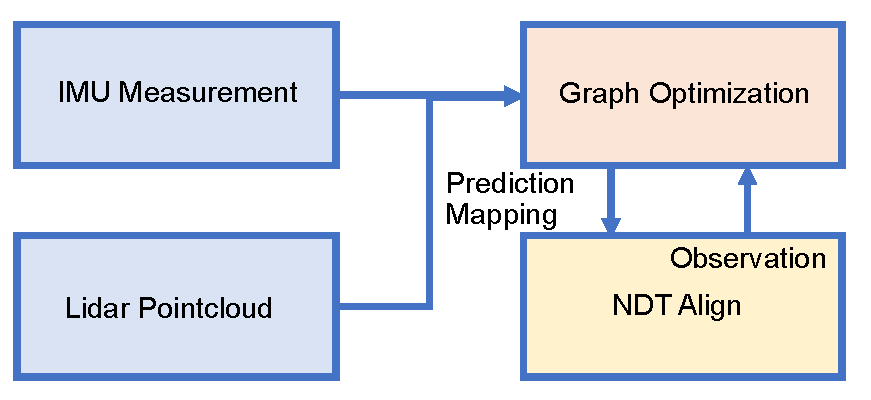
\includegraphics[width=0.4\textwidth]{resources/lio/lio-preinteg.pdf}
	\caption{Computational framework of preintegrated LIO}
	\label{fig:framework-lio-preinteg}
\end{figure}

\subsection{Code Implementation}  
The code in this section is primarily built upon Section~\ref{sec:iekf-lio} with the addition of graph optimization methods. Most of the core logic remains unchanged. The LIO system now includes a preintegrator that handles IMU data integration and provides predicted states, while also maintaining an incremental NDT odometer for point cloud registration and local map management.

\begin{lstlisting}[language=c++,caption=src/ch8/lio-preinteg/lio_preinteg.h]
class LioPreinteg {
	private:
	/// modules
	std::shared_ptr<MessageSync> sync_ = nullptr;
	StaticIMUInit imu_init_;
	
	/// point clouds data
	FullCloudPtr scan_undistort_{new FullPointCloudType()};  // scan after undistortion
	CloudPtr current_scan_ = nullptr;
	
	// optimization-related
	NavStated last_nav_state_, current_nav_state_;  // previous and current states  
	Mat15d prior_info_ = Mat15d::Identity();        // prior constraint
	std::shared_ptr<IMUPreintegration> preinteg_ = nullptr;
	
	IMUPtr last_imu_ = nullptr;
	
	/// NDT data
	IncNdt3d ndt_;
	SE3 ndt_pose_;
	SE3 last_ndt_pose_;
	
	Options options_;
	std::shared_ptr<ui::PangolinWindow> ui_ = nullptr;
};
\end{lstlisting}

During the prediction phase, we use poses from preintegration to undistort point clouds:

\begin{lstlisting}[language=c++,caption=src/ch8/lio-preinteg/lio_preinteg.cc]
void LioPreinteg::Predict() {
	imu_states_.clear();
	imu_states_.emplace_back(last_nav_state_);
	
	/// Predict IMU states
	for (auto &imu : measures_.imu_) {
		if (last_imu_ != nullptr) {
			preinteg_->Integrate(*imu, imu->timestamp_ - last_imu_->timestamp_);
		}
		
		last_imu_ = imu;
		imu_states_.emplace_back(preinteg_->Predict(last_nav_state_, imu_init_.GetGravity()));
	}
}
\end{lstlisting}

During registration, the predicted pose from preintegration is used as input to the NDT odometer, while the NDT output serves as observations for optimization:

\begin{lstlisting}[language=c++,caption=src/ch8/lio-preinteg/lio_preinteg.cc]
void LioPreinteg::Align() {
	LOG(INFO) << "=== frame " << frame_num_;
	ndt_.SetSource(current_scan_filter_);
	
	current_nav_state_ = preinteg_->Predict(last_nav_state_, imu_init_.GetGravity());
	ndt_pose_ = current_nav_state_.GetSE3();
	
	ndt_.AlignNdt(ndt_pose_);
	
	Optimize();
}

void LioPreinteg::Optimize() {
	using BlockSolverType = g2o::BlockSolverX;
	using LinearSolverType = g2o::LinearSolverEigen<BlockSolverType::PoseMatrixType>;
	
	auto *solver = new g2o::OptimizationAlgorithmLevenberg(
	g2o::make_unique<BlockSolverType>(g2o::make_unique<LinearSolverType>()));
	g2o::SparseOptimizer optimizer;
	optimizer.setAlgorithm(solver);
	
	// Previous frame vertices: pose, v, bg, ba
	auto v0_pose = new VertexPose();
	v0_pose->setId(0);
	v0_pose->setEstimate(last_nav_state_.GetSE3());
	optimizer.addVertex(v0_pose);
	
	auto v0_vel = new VertexVelocity();
	v0_vel->setId(1);
	v0_vel->setEstimate(last_nav_state_.v_);
	optimizer.addVertex(v0_vel);
	
	auto v0_bg = new VertexGyroBias();
	v0_bg->setId(2);
	v0_bg->setEstimate(last_nav_state_.bg_);
	optimizer.addVertex(v0_bg);
	
	auto v0_ba = new VertexAccBias();
	v0_ba->setId(3);
	v0_ba->setEstimate(last_nav_state_.ba_);
	optimizer.addVertex(v0_ba);
	
	// Current frame vertices: pose, v, bg, ba
	auto v1_pose = new VertexPose();
	v1_pose->setId(4);
	v1_pose->setEstimate(ndt_pose_);  // NDT pose as initial value
	optimizer.addVertex(v1_pose);
	
	auto v1_vel = new VertexVelocity();
	v1_vel->setId(5);
	v1_vel->setEstimate(current_nav_state_.v_);
	optimizer.addVertex(v1_vel);
	
	auto v1_bg = new VertexGyroBias();
	v1_bg->setId(6);
	v1_bg->setEstimate(current_nav_state_.bg_);
	optimizer.addVertex(v1_bg);
	
	auto v1_ba = new VertexAccBias();
	v1_ba->setId(7);
	v1_ba->setEstimate(current_nav_state_.ba_);
	optimizer.addVertex(v1_ba);
	
	// IMU factor
	auto edge_inertial = new EdgeInertial(preinteg_, imu_init_.GetGravity());
	edge_inertial->setVertex(0, v0_pose);
	edge_inertial->setVertex(1, v0_vel);
	edge_inertial->setVertex(2, v0_bg);
	edge_inertial->setVertex(3, v0_ba);
	edge_inertial->setVertex(4, v1_pose);
	edge_inertial->setVertex(5, v1_vel);
	auto *rk = new g2o::RobustKernelHuber();
	rk->setDelta(200.0);
	edge_inertial->setRobustKernel(rk);
	optimizer.addEdge(edge_inertial);
	
	// Bias random walk
	auto *edge_gyro_rw = new EdgeGyroRW();
	edge_gyro_rw->setVertex(0, v0_bg);
	edge_gyro_rw->setVertex(1, v1_bg);
	edge_gyro_rw->setInformation(options_.bg_rw_info_);
	optimizer.addEdge(edge_gyro_rw);
	
	auto *edge_acc_rw = new EdgeAccRW();
	edge_acc_rw->setVertex(0, v0_ba);
	edge_acc_rw->setVertex(1, v1_ba);
	edge_acc_rw->setInformation(options_.ba_rw_info_);
	optimizer.addEdge(edge_acc_rw);
	
	// Prior for previous frame pose, vel, bg, ba
	auto *edge_prior = new EdgePriorPoseNavState(last_nav_state_, prior_info_);
	edge_prior->setVertex(0, v0_pose);
	edge_prior->setVertex(1, v0_vel);
	edge_prior->setVertex(2, v0_bg);
	edge_prior->setVertex(3, v0_ba);
	optimizer.addEdge(edge_prior);
	
	/// NDT pose observation
	auto *edge_ndt = new EdgeGNSS(v1_pose, ndt_pose_);
	edge_ndt->setInformation(options_.ndt_info_);
	optimizer.addEdge(edge_ndt);
	
	// Optimization
	optimizer.setVerbose(options_.verbose_);
	optimizer.initializeOptimization();
	optimizer.optimize(20);
	
	// Get results
	last_nav_state_.R_ = v0_pose->estimate().so3();
	last_nav_state_.p_ = v0_pose->estimate().translation();
	last_nav_state_.v_ = v0_vel->estimate();
	last_nav_state_.bg_ = v0_bg->estimate();
	last_nav_state_.ba_ = v0_ba->estimate();
	
	current_nav_state_.R_ = v1_pose->estimate().so3();
	current_nav_state_.p_ = v1_pose->estimate().translation();
	current_nav_state_.v_ = v1_vel->estimate();
	current_nav_state_.bg_ = v1_bg->estimate();
	current_nav_state_.ba_ = v1_ba->estimate();
	
	/// Reset preintegration
	
	options_.preinteg_options_.init_bg_ = current_nav_state_.bg_;
	options_.preinteg_options_.init_ba_ = current_nav_state_.ba_;
	preinteg_ = std::make_shared<IMUPreintegration>(options_.preinteg_options_);
	
	// Compute prior for current frame
	// Build Hessian
	// 15x2, order: v0_pose, v0_vel, v0_bg, v0_ba, v1_pose, v1_vel, v1_bg, v1_ba
	//            0       6        9     12     15        21      24     27
	Eigen::Matrix<double, 30, 30> H;
	H.setZero();
	
	H.block<24, 24>(0, 0) += edge_inertial->GetHessian();
	
	Eigen::Matrix<double, 6, 6> Hgr = edge_gyro_rw->GetHessian();
	H.block<3, 3>(9, 9) += Hgr.block<3, 3>(0, 0);
	H.block<3, 3>(9, 24) += Hgr.block<3, 3>(0, 3);
	H.block<3, 3>(24, 9) += Hgr.block<3, 3>(3, 0);
	H.block<3, 3>(24, 24) += Hgr.block<3, 3>(3, 3);
	
	Eigen::Matrix<double, 6, 6> Har = edge_acc_rw->GetHessian();
	H.block<3, 3>(12, 12) += Har.block<3, 3>(0, 0);
	H.block<3, 3>(12, 27) += Har.block<3, 3>(0, 3);
	H.block<3, 3>(27, 12) += Har.block<3, 3>(3, 0);
	H.block<3, 3>(27, 27) += Har.block<3, 3>(3, 3);
	
	H.block<15, 15>(0, 0) += edge_prior->GetHessian();
	H.block<6, 6>(15, 15) += edge_ndt->GetHessian();
	
	H = math::Marginalize(H, 0, 14);
	prior_info_ = H.block<15, 15>(15, 15);
	
	if (options_.verbose_) {
		LOG(INFO) << "info trace: " << prior_info_.trace();
		LOG(INFO) << "optimization done.";
	}
	
	NormalizeVelocity();
	last_nav_state_ = current_nav_state_;
}
\end{lstlisting}

Most of the code here is dedicated to constructing the graph optimization structure, which corresponds to Figure~\ref{fig:preinteg-graph}. In our implementation, the graph optimization problem for two keyframes consists of 8 vertices, 1 preintegration edge, 2 random walk edges, 1 NDT posterior pose observation, and 1 prior constraint. We didn't directly formulate the NDT observation in graph optimization form because NDT requires updating nearest neighbors during iteration, which isn't directly supported by g2o. After each optimization, we marginalize the previous frame's state. Since g2o doesn't directly support marginalization, we manually assemble the complete Hessian matrix using each edge's Jacobian matrices, which are computed during linearization.

\begin{lstlisting}[language=c++,caption=src/common/g2o_types.h]
class EdgePriorPoseNavState : public g2o::BaseMultiEdge<15, Vec15d> {
	public:
	void computeError();
	virtual void linearizeOplus();
	
	Eigen::Matrix<double, 15, 15> GetHessian() {
		linearizeOplus();
		Eigen::Matrix<double, 15, 15> J;
		J.block<15, 6>(0, 0) = _jacobianOplus[0];
		J.block<15, 3>(0, 6) = _jacobianOplus[1];
		J.block<15, 3>(0, 9) = _jacobianOplus[2];
		J.block<15, 3>(0, 12) = _jacobianOplus[3];
		return J.transpose() * information() * J;
	}
	
	NavStated state_;
};
\end{lstlisting}

Finally, we process the $\mathbf{H}$ matrix with the math::Marginalize function to marginalize rows 0-14, obtaining the information matrix (15×15 dimension) for the next frame's state. This matrix is then used as prior information in the next optimization problem. Running the test\_lio\_preinteg program displays the LIO's real-time point cloud, as shown in Figure~\ref{fig:lio-preinteg}.

\begin{figure}[!htp]
	\centering
	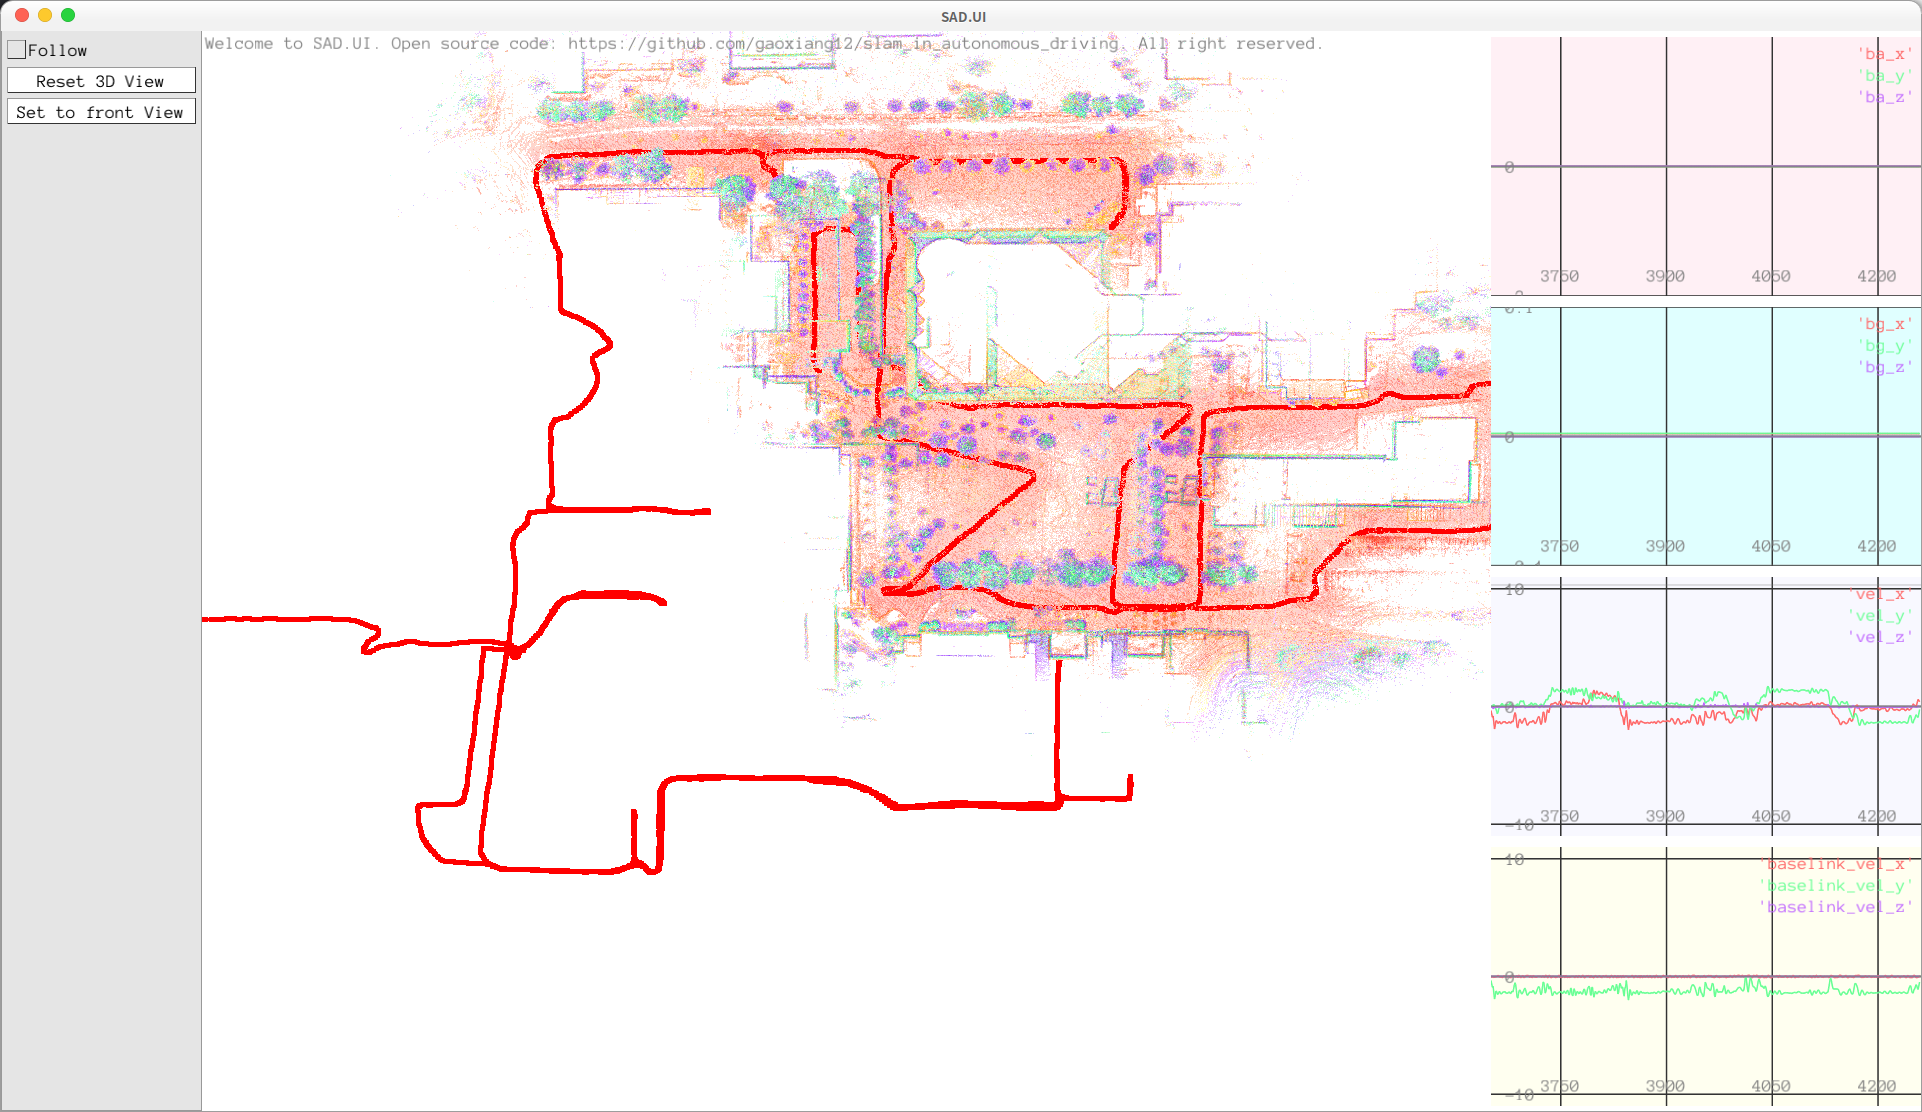
\includegraphics[width=0.8\textwidth]{resources/lio/lio-preinteg.png}
	\caption{Preintegration-based LIO system}
	\label{fig:lio-preinteg}
\end{figure}

The preintegration optimization demonstrated in this section primarily operates between consecutive LiDAR scans. Readers may modify it to accumulate over longer periods to better highlight differences between preintegration and filtering methods, which we leave as an exercise.

\section{Summary}  
This section introduced the tightly-coupled LIO system to the readers. We presented two approaches: the iterative Kalman filter-based method and the pre-integration nonlinear optimization-based method. Overall, both methods work effectively. There is no significant difference in the point cloud quality during normal operation, but the actual debugging difficulty varies. The implementation of the pre-integration system is noticeably more complex. If desired, each NDT registration can be configured as a graph optimization factor to achieve a truly tightly-coupled system, but that would also entail more extensive debugging. We hope readers can gain an understanding of the frontend and backend workings of a tightly-coupled system through the content of this chapter.  

\section*{Exercises}  
\begin{enumerate}  
	\item Referring to the derivation of NDT-based LIO, derive the Kalman update formula for LIO based on point-to-plane residuals, and explain the relationship between point-to-plane ICP and LIO.  
	\item Investigate whether the matrices computed by NDT in NDT LIO contain a significant number of zero blocks. If the goal is to reduce the matrix size, can these zero blocks be removed, retaining only the non-zero blocks?  
	\item In the pre-integration LIO system, increase the pre-integration time—for example, marginalize only after more than 3 seconds instead of after processing each frame.  
	\item *Incorporate NDT residuals into the pre-integration system to implement an LIO system.  
\end{enumerate}

